% Options for packages loaded elsewhere
\PassOptionsToPackage{unicode}{hyperref}
\PassOptionsToPackage{hyphens}{url}
\PassOptionsToPackage{dvipsnames,svgnames,x11names}{xcolor}
%
\documentclass[
  12pt,
]{interact}

\usepackage{amsmath,amssymb}
\usepackage{setspace}
\usepackage{iftex}
\ifPDFTeX
  \usepackage[T1]{fontenc}
  \usepackage[utf8]{inputenc}
  \usepackage{textcomp} % provide euro and other symbols
\else % if luatex or xetex
  \usepackage{unicode-math}
  \defaultfontfeatures{Scale=MatchLowercase}
  \defaultfontfeatures[\rmfamily]{Ligatures=TeX,Scale=1}
\fi
\usepackage{lmodern}
\ifPDFTeX\else  
    % xetex/luatex font selection
\fi
% Use upquote if available, for straight quotes in verbatim environments
\IfFileExists{upquote.sty}{\usepackage{upquote}}{}
\IfFileExists{microtype.sty}{% use microtype if available
  \usepackage[]{microtype}
  \UseMicrotypeSet[protrusion]{basicmath} % disable protrusion for tt fonts
}{}
\makeatletter
\@ifundefined{KOMAClassName}{% if non-KOMA class
  \IfFileExists{parskip.sty}{%
    \usepackage{parskip}
  }{% else
    \setlength{\parindent}{0pt}
    \setlength{\parskip}{6pt plus 2pt minus 1pt}}
}{% if KOMA class
  \KOMAoptions{parskip=half}}
\makeatother
\usepackage{xcolor}
\setlength{\emergencystretch}{3em} % prevent overfull lines
\setcounter{secnumdepth}{5}
% Make \paragraph and \subparagraph free-standing
\makeatletter
\ifx\paragraph\undefined\else
  \let\oldparagraph\paragraph
  \renewcommand{\paragraph}{
    \@ifstar
      \xxxParagraphStar
      \xxxParagraphNoStar
  }
  \newcommand{\xxxParagraphStar}[1]{\oldparagraph*{#1}\mbox{}}
  \newcommand{\xxxParagraphNoStar}[1]{\oldparagraph{#1}\mbox{}}
\fi
\ifx\subparagraph\undefined\else
  \let\oldsubparagraph\subparagraph
  \renewcommand{\subparagraph}{
    \@ifstar
      \xxxSubParagraphStar
      \xxxSubParagraphNoStar
  }
  \newcommand{\xxxSubParagraphStar}[1]{\oldsubparagraph*{#1}\mbox{}}
  \newcommand{\xxxSubParagraphNoStar}[1]{\oldsubparagraph{#1}\mbox{}}
\fi
\makeatother


\providecommand{\tightlist}{%
  \setlength{\itemsep}{0pt}\setlength{\parskip}{0pt}}\usepackage{longtable,booktabs,array}
\usepackage{calc} % for calculating minipage widths
% Correct order of tables after \paragraph or \subparagraph
\usepackage{etoolbox}
\makeatletter
\patchcmd\longtable{\par}{\if@noskipsec\mbox{}\fi\par}{}{}
\makeatother
% Allow footnotes in longtable head/foot
\IfFileExists{footnotehyper.sty}{\usepackage{footnotehyper}}{\usepackage{footnote}}
\makesavenoteenv{longtable}
\usepackage{graphicx}
\makeatletter
\def\maxwidth{\ifdim\Gin@nat@width>\linewidth\linewidth\else\Gin@nat@width\fi}
\def\maxheight{\ifdim\Gin@nat@height>\textheight\textheight\else\Gin@nat@height\fi}
\makeatother
% Scale images if necessary, so that they will not overflow the page
% margins by default, and it is still possible to overwrite the defaults
% using explicit options in \includegraphics[width, height, ...]{}
\setkeys{Gin}{width=\maxwidth,height=\maxheight,keepaspectratio}
% Set default figure placement to htbp
\makeatletter
\def\fps@figure{htbp}
\makeatother
% definitions for citeproc citations
\NewDocumentCommand\citeproctext{}{}
\NewDocumentCommand\citeproc{mm}{%
  \begingroup\def\citeproctext{#2}\cite{#1}\endgroup}
\makeatletter
 % allow citations to break across lines
 \let\@cite@ofmt\@firstofone
 % avoid brackets around text for \cite:
 \def\@biblabel#1{}
 \def\@cite#1#2{{#1\if@tempswa , #2\fi}}
\makeatother
\newlength{\cslhangindent}
\setlength{\cslhangindent}{1.5em}
\newlength{\csllabelwidth}
\setlength{\csllabelwidth}{3em}
\newenvironment{CSLReferences}[2] % #1 hanging-indent, #2 entry-spacing
 {\begin{list}{}{%
  \setlength{\itemindent}{0pt}
  \setlength{\leftmargin}{0pt}
  \setlength{\parsep}{0pt}
  % turn on hanging indent if param 1 is 1
  \ifodd #1
   \setlength{\leftmargin}{\cslhangindent}
   \setlength{\itemindent}{-1\cslhangindent}
  \fi
  % set entry spacing
  \setlength{\itemsep}{#2\baselineskip}}}
 {\end{list}}
\usepackage{calc}
\newcommand{\CSLBlock}[1]{\hfill\break\parbox[t]{\linewidth}{\strut\ignorespaces#1\strut}}
\newcommand{\CSLLeftMargin}[1]{\parbox[t]{\csllabelwidth}{\strut#1\strut}}
\newcommand{\CSLRightInline}[1]{\parbox[t]{\linewidth - \csllabelwidth}{\strut#1\strut}}
\newcommand{\CSLIndent}[1]{\hspace{\cslhangindent}#1}

\usepackage{booktabs}
\usepackage{longtable}
\usepackage{array}
\usepackage{multirow}
\usepackage{wrapfig}
\usepackage{float}
\usepackage{colortbl}
\usepackage{pdflscape}
\usepackage{tabu}
\usepackage{threeparttable}
\usepackage{threeparttablex}
\usepackage[normalem]{ulem}
\usepackage{makecell}
\usepackage{xcolor}
\usepackage{orcidlink}
\usepackage{algorithm}
\usepackage{float}
\usepackage{amsmath}
\usepackage{amsthm}
\usepackage{amssymb}
\theoremstyle{plain}
\newtheorem{assumption}{\protect\assumptionname}
\newtheorem{claim}{\protect\claimname}
\newtheorem{condition}{\protect\conditionname}
\newtheorem{conjecture}{\protect\conjecturename}
\newtheorem{cor}{\protect\corollaryname}
\newtheorem{defn}{\protect\definitionname}
\newtheorem{example}{\protect\examplename}
\newtheorem{lem}{\protect\lemmaname}
\newtheorem{notation}{\protect\notationname}
\newtheorem{problem}{\protect\problemname}
\newtheorem{prop}{\protect\propositionname}
\newtheorem{rem}{\protect\remarkname}
\newtheorem{thm}{\protect\theoremname}
\providecommand{\assumptionname}{Assumption}
\providecommand{\claimname}{Claim}
\providecommand{\conditionname}{Condition}
\providecommand{\conjecturename}{Conjecture}
\providecommand{\corollaryname}{Corollary}
\providecommand{\definitionname}{Definition}
\providecommand{\examplename}{Example}
\providecommand{\lemmaname}{Lemma}
\providecommand{\notationname}{Notation}
\providecommand{\problemname}{Problem}
\providecommand{\propositionname}{Proposition}
\providecommand{\remarkname}{Remark}
\providecommand{\theoremname}{Theorem}
\makeatletter
\@ifpackageloaded{tcolorbox}{}{\usepackage[skins,breakable]{tcolorbox}}
\@ifpackageloaded{fontawesome5}{}{\usepackage{fontawesome5}}
\definecolor{quarto-callout-color}{HTML}{909090}
\definecolor{quarto-callout-note-color}{HTML}{0758E5}
\definecolor{quarto-callout-important-color}{HTML}{CC1914}
\definecolor{quarto-callout-warning-color}{HTML}{EB9113}
\definecolor{quarto-callout-tip-color}{HTML}{00A047}
\definecolor{quarto-callout-caution-color}{HTML}{FC5300}
\definecolor{quarto-callout-color-frame}{HTML}{acacac}
\definecolor{quarto-callout-note-color-frame}{HTML}{4582ec}
\definecolor{quarto-callout-important-color-frame}{HTML}{d9534f}
\definecolor{quarto-callout-warning-color-frame}{HTML}{f0ad4e}
\definecolor{quarto-callout-tip-color-frame}{HTML}{02b875}
\definecolor{quarto-callout-caution-color-frame}{HTML}{fd7e14}
\makeatother
\makeatletter
\@ifpackageloaded{caption}{}{\usepackage{caption}}
\AtBeginDocument{%
\ifdefined\contentsname
  \renewcommand*\contentsname{Table of contents}
\else
  \newcommand\contentsname{Table of contents}
\fi
\ifdefined\listfigurename
  \renewcommand*\listfigurename{List of Figures}
\else
  \newcommand\listfigurename{List of Figures}
\fi
\ifdefined\listtablename
  \renewcommand*\listtablename{List of Tables}
\else
  \newcommand\listtablename{List of Tables}
\fi
\ifdefined\figurename
  \renewcommand*\figurename{Figure}
\else
  \newcommand\figurename{Figure}
\fi
\ifdefined\tablename
  \renewcommand*\tablename{Table}
\else
  \newcommand\tablename{Table}
\fi
}
\@ifpackageloaded{float}{}{\usepackage{float}}
\floatstyle{ruled}
\@ifundefined{c@chapter}{\newfloat{codelisting}{h}{lop}}{\newfloat{codelisting}{h}{lop}[chapter]}
\floatname{codelisting}{Listing}
\newcommand*\listoflistings{\listof{codelisting}{List of Listings}}
\makeatother
\makeatletter
\makeatother
\makeatletter
\@ifpackageloaded{caption}{}{\usepackage{caption}}
\@ifpackageloaded{subcaption}{}{\usepackage{subcaption}}
\makeatother

\ifLuaTeX
  \usepackage{selnolig}  % disable illegal ligatures
\fi
\usepackage{bookmark}

\IfFileExists{xurl.sty}{\usepackage{xurl}}{} % add URL line breaks if available
\urlstyle{same} % disable monospaced font for URLs
\hypersetup{
  pdftitle={New Metrics for Assessing Projection Pursuit Indexes, and Guiding Optimisation Choices},
  pdfauthor={H. Sherry Zhang; Dianne Cook; Nicolas Langrené; Jessica Wai Yin Leung},
  pdfkeywords={projection pursuit, jellyfish search optimiser
(JSO), optimisation, grand tour, high-dimensional data, exploratory data
analysis},
  colorlinks=true,
  linkcolor={blue},
  filecolor={Maroon},
  citecolor={Blue},
  urlcolor={Blue},
  pdfcreator={LaTeX via pandoc}}


\title{New Metrics for Assessing Projection Pursuit Indexes, and Guiding
Optimisation Choices}
\author{H. Sherry Zhang$\textsuperscript{1}$, Dianne
Cook$\textsuperscript{2}$, Nicolas
Langrené$\textsuperscript{3}$, Jessica Wai Yin
Leung$\textsuperscript{2}$}

\thanks{CONTACT: H. Sherry
Zhang. Email: \href{mailto:huize.zhang@austin.utexas.edu}{\nolinkurl{huize.zhang@austin.utexas.edu}}. Dianne
Cook. Email: \href{mailto:dicook@monash.edu}{\nolinkurl{dicook@monash.edu}}. Nicolas
Langrené. Email: \href{mailto:nicolaslangrene@uic.edu.cn}{\nolinkurl{nicolaslangrene@uic.edu.cn}}. Jessica
Wai Yin
Leung. Email: \href{mailto:Jessica.Leung@monash.edu}{\nolinkurl{Jessica.Leung@monash.edu}}. }
\begin{document}
\captionsetup{labelsep=space}
\maketitle
\textsuperscript{1} Department of Statistics and Data
Sciences, University of Texas at Austin, Austin, United
States\\ \textsuperscript{2} Department of Econometrics and Business
Statistics, Monash
University, Melbourne, Australia\\ \textsuperscript{3} Department of
Mathematical Sciences, Guangdong Provincial Key Laboratory of
Interdisciplinary Research and Application for Data Science,
BNU-HKBU~United~International~College, Zhuhai, China
\begin{abstract}
The projection pursuit (PP) guided tour interactively optimises a
criteria function known as the PP index, to explore high-dimensional
data by revealing interesting projections. Optimisation of some PP
indexes can be non-trivial, if they are non-smooth functions, or the
optima has a small ``squint angle'', detectable only from close
proximity. To address these challenges, this study investigates the
performance of a recently introduced swarm-based algorithm, Jellyfish
Search Optimiser (JSO), for optimising PP indexes. The performance of
JSO for visualising data is evaluated across various hyper-parameter
settings and compared with existing optimisers. Additionally, methods
for calculating the smoothness and squintability properties of the PP
index are proposed. They are used to assess the optimiser performance in
the presence of PP index complexities. A simulation study illustrates
the use of these performance metrics to compare the JSO with existing
optimisation methods available for the guided tour. The JSO algorithm
has been implemented in the R package, \texttt{tourr}, and functions to
calculate smoothness and squintability are available in the
\texttt{ferrn} package.
\end{abstract}
\begin{keywords}
\def\sep{;\ }
projection pursuit\sep jellyfish search optimiser
(JSO)\sep optimisation\sep grand tour\sep high-dimensional data\sep 
exploratory data analysis
\end{keywords}


\setstretch{2}
\section{Introduction}\label{introduction}

Projection pursuit (PP) (Kruskal (1969), Friedman and Tukey (1974),
Huber (1985)) is a dimension reduction technique aimed at identifying
informative linear projections of data. This is useful for exploring
high-dimensional data, and creating plots of the data that reveal the
main features to use for publication. The method involves optimising an
objective function known as the PP index (e.g. Hall (1989), Cook, Buja,
and Cabrera (1993), Lee and Cook (2010), Loperfido (2018), Loperfido
(2020)), which defines the criteria for what constitutes interesting or
informative projections. Let \(X \in \mathbb{R}^{n\times p}\) be the
data matrix, \(A \in\mathbb{R}^{p \times d}\) be an orthonormal matrix,
where \(A\) belongs to the Stiefel manifold
\(\mathcal{A} = V_d(\mathbb{R}^p)\). The projection \(Y = XA\) is a
linear transformation that maps data from a \(p\)-dimensional space into
a \(d\)-dimensional space. The index function
\(f(XA): \mathbb{R}^{n \times d} \to \mathbb{R}\) is a scalar function
that measures an interesting aspect of the projected data, such as
deviation from normality, presence of clusters, non-linear structure, or
other features of interest. For a fixed sample of data, PP finds the
orthonormal basis \(A\) that maximises the index value of the
projection, \(Y = XA\):

\begin{equation}\phantomsection\label{eq-optimization}{
\underset{A \in \mathcal{A}}{\max } \quad f(XA) \quad \text{subject to} \quad A'A = I_d
}\end{equation}

It is interesting to note that when using PP visually, one cares less
about \(A\) than the plane described by \(A\), because the orientation
in the plane is irrelevant. The space of planes belongs to a Grassmann
manifold. This is usually how the projection pursuit guided tour (PPGT)
(Cook et al. 1995) operates, when using geodesic interpolation between
starting and target planes. It interpolates plane to plane, removing
irrelevant within plane spin, and is agnostic to the basis (\(A\)) used
to define the plane. Thus, indexes which are used for the PPGT should be
rotationally invariant.

Index functions are quite varied in form, partially depending on the
data that is being projected. Figure~\ref{fig-example-functions} shows
two examples. Huber plots (Huber 1990) of 2D data sets are in (a) and
(c), showing the PP index values for all 1D projections of the 2D data
in polar coordinates, which reveals the form of these functions. The
dashed circle is a baseline set at the average value, and the straight
line marks the optimal projection. Plots (b) and (d) show the respective
best projections of the data as histograms. Indexes like the holes,
central mass and skewness (Cook, Buja, and Cabrera 1993) are generally
smooth for most data sets, but capture only large patterns. Many indexes
noisy and non-convex, requiring an effective and efficient optimisation
procedure to explore the data landscape and achieve a globally optimal
viewpoint of the data. The skewness index computed for trimodal data, in
(a), is smooth with a large squint angle but has three modes, and thus
is not convex. The binned normality index (a simple version of a
non-normality index as described in Huber (1985)) computed on the famous
RANDU data, in (c), is noisier and has a very small squint angle. The
discreteness cannot be seen unless the optimiser is very close to the
optimal projection.

\begin{figure}

\centering{

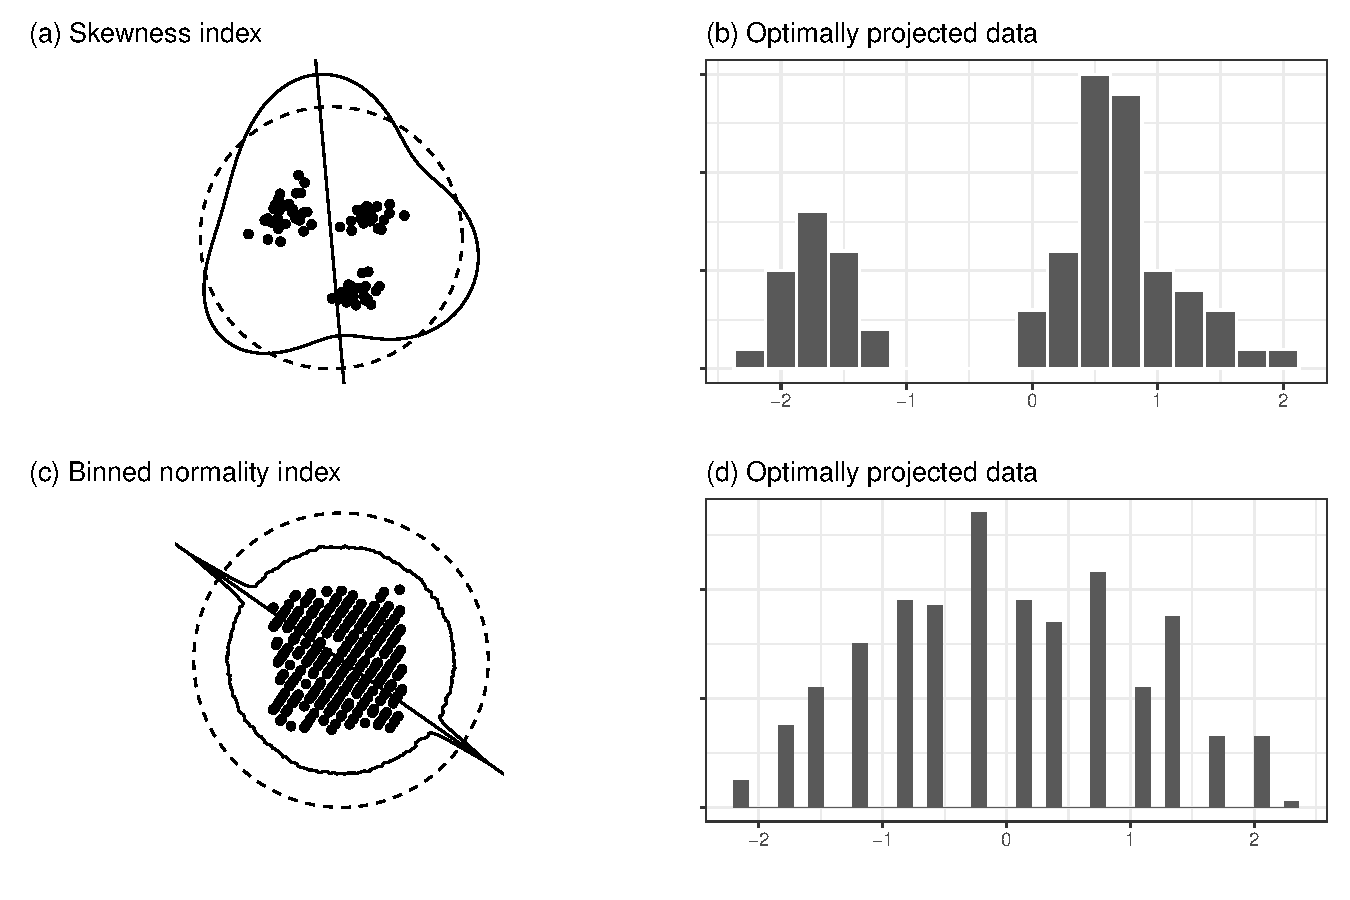
\includegraphics[width=0.8\textwidth,height=\textheight]{jso_files/figure-pdf/fig-example-functions-1.pdf}

}

\caption{\label{fig-example-functions}Examples of PP indexes with large
(top row) and small (bottom row) squint angles, shown with a Huber plot,
and histogram of the projected data corresponding to the optimal
projection. A Huber plot shows the PP index values for all 1D data
projections in polar coordinates.}

\end{figure}%

Optimisation of PP is often discussed when new indexes are proposed
(Posse 1995a; Marie-Sainte, Berro, and Ruiz-Gazen 2010; Grochowski and
Duch 2011). Cook et al. (1995) tied the optimisation more closely to the
index, when they introduced the PPGT, which monitors the optimisation
visually so that the user can see the projected data leading in and out
of the optima. An implementation is available in the \texttt{tourr}
package (Wickham et al. 2011) in R (R Core Team 2023). Zhang et al.
(2021) illustrated how to diagnose optimisation processes, particularly
focusing on the guided tour, and revealed a need for improved
optimisation. While improving the quality of the optimisation solutions
in the tour is essential, it is also important to be able to view the
data projections as the optimisation progresses. Integrating the guided
tour with a global optimisation algorithm that is efficient in finding
the global optimal and enables viewing of the projected data during the
exploration process is a goal.

Here, the potential for a Jellyfish Search Optimiser (JSO) (see Chou and
Truong (2021), and Rajwar, Deep, and Das (2023)) for the PPGT is
explored. JSO, inspired by the search behaviour of jellyfish in the
ocean, is a swarm-based metaheuristic designed to solve global
optimisation problems. Compared to traditional methods, JSO has
demonstrated stronger search ability and faster convergence, and
requires fewer tuning parameters. These practicalities make JSO a
promising candidate for enhancing PP optimisation.

The primary goal of the study reported here is to investigate the
performance of JSO in PP optimisation for the guided tour. It is of
interest to assess how quickly and closely the optimiser reaches a gobal
optima, for various PP indexes that may have differing complexities. To
observe the performance of JSO with different types of PP indexes,
metrics are introduced to capture specific properties of the index
including squintability (based on Tukey and Tukey (1981)'s squint angle)
and smoothness. Here, we mathematically define metrics for squintability
and smoothness, which is a new contribution for PP research. A series of
simulation experiments using various datasets and PP indexes are
conducted to assess JSO's behaviour and its sensitivity to
hyper-parameter choices (number of jellyfish and maximum number of
tries). The relationship between the JSO performance, hyper-parameter
choices and properties of PP indexes (smoothness and squintability) is
analysed to provide guidance on selecting optimisers for practitioners
using projection pursuit. Additionally, this work should guide the
design of new PP indexes and facilitate better optimization for PP.

The paper is structured as follows. Section~\ref{sec-background}
introduces the background of the PPGT, reviews existing optimisers and
index functions in the literature. Section~\ref{sec-PP-properties}
introduces the metrics that measure different properties of PP indexes,
smoothness and squintability, and Section~\ref{sec-JSO} describes the
new JSO to be used for the PPGT. Section~\ref{sec-sim-deets} summarises
the results of two simulation experiments done to assess JSO's
performance: one comparing JSO's performance improvements relative to an
existing optimiser, Creeping Random Search (CRS), and the other studying
the impact of different PP index properties on optimisation performance.
Section~\ref{sec-sim-res} presents the results.
Section~\ref{sec-discussion} discusses implementation details and
insights for practitioners. Section~\ref{sec-conclusion} summarises the
work and provides suggestions for future directions.

\section{Projection pursuit, tours, index functions and
optimisation}\label{sec-background}

A tour on high-dimensional data is constructed by geodesically
interpolating between pairs of planes. Any plane is described by an
orthonormal basis, \(A_t\), where \(t\) represents time in the sequence.
The term ``geodesic'' refers to maintaining the orthonormality
constraint so that each view shown is correctly a projection of the
data. The PP guided tour operates by geodesically interpolating to
target planes (projections) which have high PP index values, as provided
by the optimiser. The geodesic interpolation means that the viewer sees
a continuous sequence of projections of the data, so they can watch
patterns of interest forming as the function is optimised. There are
five optimisation methods implemented in the \texttt{tourr} package:

\begin{itemize}
\tightlist
\item
  a pseudo-derivative, that searches locally for the best direction,
  based on differencing the index values for very close projections.
\item
  a brute-force optimisation (CRS).
\item
  a modified brute force algorithm described in Posse (1995b).
\item
  an essentially simulated annealing (Bertsimas and Tsitsiklis 1993)
  where the search space is reduced as the optimisation.
\item
  a very localised search, to take tiny steps to get closer to the local
  maximum.
\end{itemize}

There are numerous PP index functions available: introduced in Cook,
Buja, and Cabrera (1993), Lee et al. (2005), Lee and Cook (2010), Grimm
(2016), Huber (1985), Ursula Laa and Valencia (2022). Most are
relatively simply defined, for any projection dimension, and implemented
because they are relatively easy to optimise. A goal is to develop PP
indexes based on scagnostics (L. Wilkinson, Anand, and Grossman (2005),
Leland Wilkinson and Wills (2008)), but the blockage is optimisation
that these tend to be noisy, with potentially small squint angles.

An initial investigation of PP indexes, and the potential for
scagnostics is described in Laa and Cook (2020). To be useful here an
optimiser needs to be able to handle index functions which are possibly
not very smooth. In addition, because data structures might be
relatively fine, the optimiser needs to be able to find maxima that
occur with a small squint angle, that can only be seen from very close
by. One last aspect that is useful is for an optimiser to return local
maxima in addition to global because data can contain many different and
interesting features.

\section{Properties of PP indexes}\label{sec-PP-properties}

Laa and Cook (2020) has proposed five criteria for assessing projection
pursuit indexes (smoothness, squintability, flexibility, rotation
invariance, and speed). Since not all index properties affect the
optimisation process, the focus here is on the first two properties,
\emph{smoothness} (Section~\ref{sec-smoothness}) and
\emph{squintability} (Section~\ref{sec-squintability}), for which
metrics are proposed to quantify them.

\subsection{Smoothness}\label{sec-smoothness}

This subsection proposes a metric for the smoothness of a projection
pursuit index.

A classical way to describe the smoothness of a function is to identify
how many continuous derivatives of the function exist. This can be
characterized by Sobolev spaces (Adams and Fournier 2003).

\begin{defn}\label{def:sobolev_space}
The Sobolev space $W^{k,p}(\mathbb{R})$ for $1\leq p\leq \infty$ is the set of all functions $f$ in $L^p(\mathbb{R})$ for which all weak derivatives $f^{(\ell)}$ of order $\ell\leq k$ exist and have a finite $L^p$ norm.
\end{defn}

The Sobolev index \(k\) in Definition \ref{def:sobolev_space} can be
used to characterize the smoothness of a function: if \(f\in W^{k,p}\),
then the higher \(k\), the smoother \(f\). While this Sobolev index
\(k\) is a useful measure of smoothness, it can be difficult to compute
or even estimate in practice.

To obtain a computable estimator of the smoothness of the index function
\(f\), we propose an approach based on random fields. If a PP index
function \(f\) is evaluated at some random bases, as is done at the
initialization stage of JSO, then these random index values can be
interpreted as a random field, indexed by a space parameter, namely the
random projection basis. This analogy suggests to use this random
training sample to fit a spatial model. We propose to use a Gaussian
process equipped with a Matérn covariance function, due to the
connections between this model and Sobolev spaces, see for example Porcu
et al. (2024).

The distribution of a Gaussian process is fully determined by its mean
and covariance function. The smoothness property comes into play in the
definition of the covariance function: if a PP index is very smooth,
then two close projection bases should produce close index values
(strong correlation); by contrast, if a PP index is not very smooth,
then two close projection bases might give very different index values
(fast decay of correlations with respect to distance between bases).
Popular covariance functions are parametric positive semi-definite
functions. In particular, the Matérn class of covariance functions has a
dedicated parameter to capture the smoothness of the Gaussian field.

\begin{defn}
The Matérn covariance function $K$ is defined by
\begin{equation}
K(u)=K_{\nu,\eta,\ell}(u):=\eta^2\frac{\left(\sqrt{2\nu}\frac{u}{\ell}\right)^{\nu}}{\Gamma(\nu)2^{\nu-1}}\mathcal{K}_{\nu}\left(\sqrt{2\nu}\frac{u}{\ell}\right)\ , u\geq0\label{eq:matern}
\end{equation}
where $\nu>0$ is the smoothness parameter, $\eta$ is the outputscale, $\ell$ is the lengthscale, and $\mathcal{K}_\nu$ is
the modified Bessel function [DLMF 10.25]. A multivariate extension $K(u)$, $u\in\mathbb{R}^d$ can be obtained by products of univariate covariance functions \eqref{eq:matern}.
\end{defn}

The Matérn covariance function can be expressed analytically when
\(\nu\) is a half-integer, the most popular values in the literature
being \(\frac{1}{2}\), \(\frac{3}{2}\) and \(\frac{5}{2}\) (Rasmussen
and Williams 2006). The parameter \(\nu\), called \emph{smoothness
parameter}, controls the decay of the covariance function. As such, it
is an appropriate measure of smoothness of a random field, as shown by
the simulations on Figure~\ref{fig-matern-1d} and
Figure~\ref{fig-matern-2d}. For example, Karvonen (2023) showed that if
a function \(f\) has a Sobolev index of \(k\), then the smoothness
parameter estimate \(\nu\) in \eqref{eq:matern} cannot be asymptotically
less than \(k\). See the survey Porcu et al. (2024) for additional
results on the connection between the Matérn model and Sobolev spaces.
An interesting result is that the asymptotic case
\(\nu\rightarrow\infty\) coincides with the Gaussian kernel:
\(K_\infty(u)=\exp(-u^{2}/2)\).

\begin{figure}

\centering{

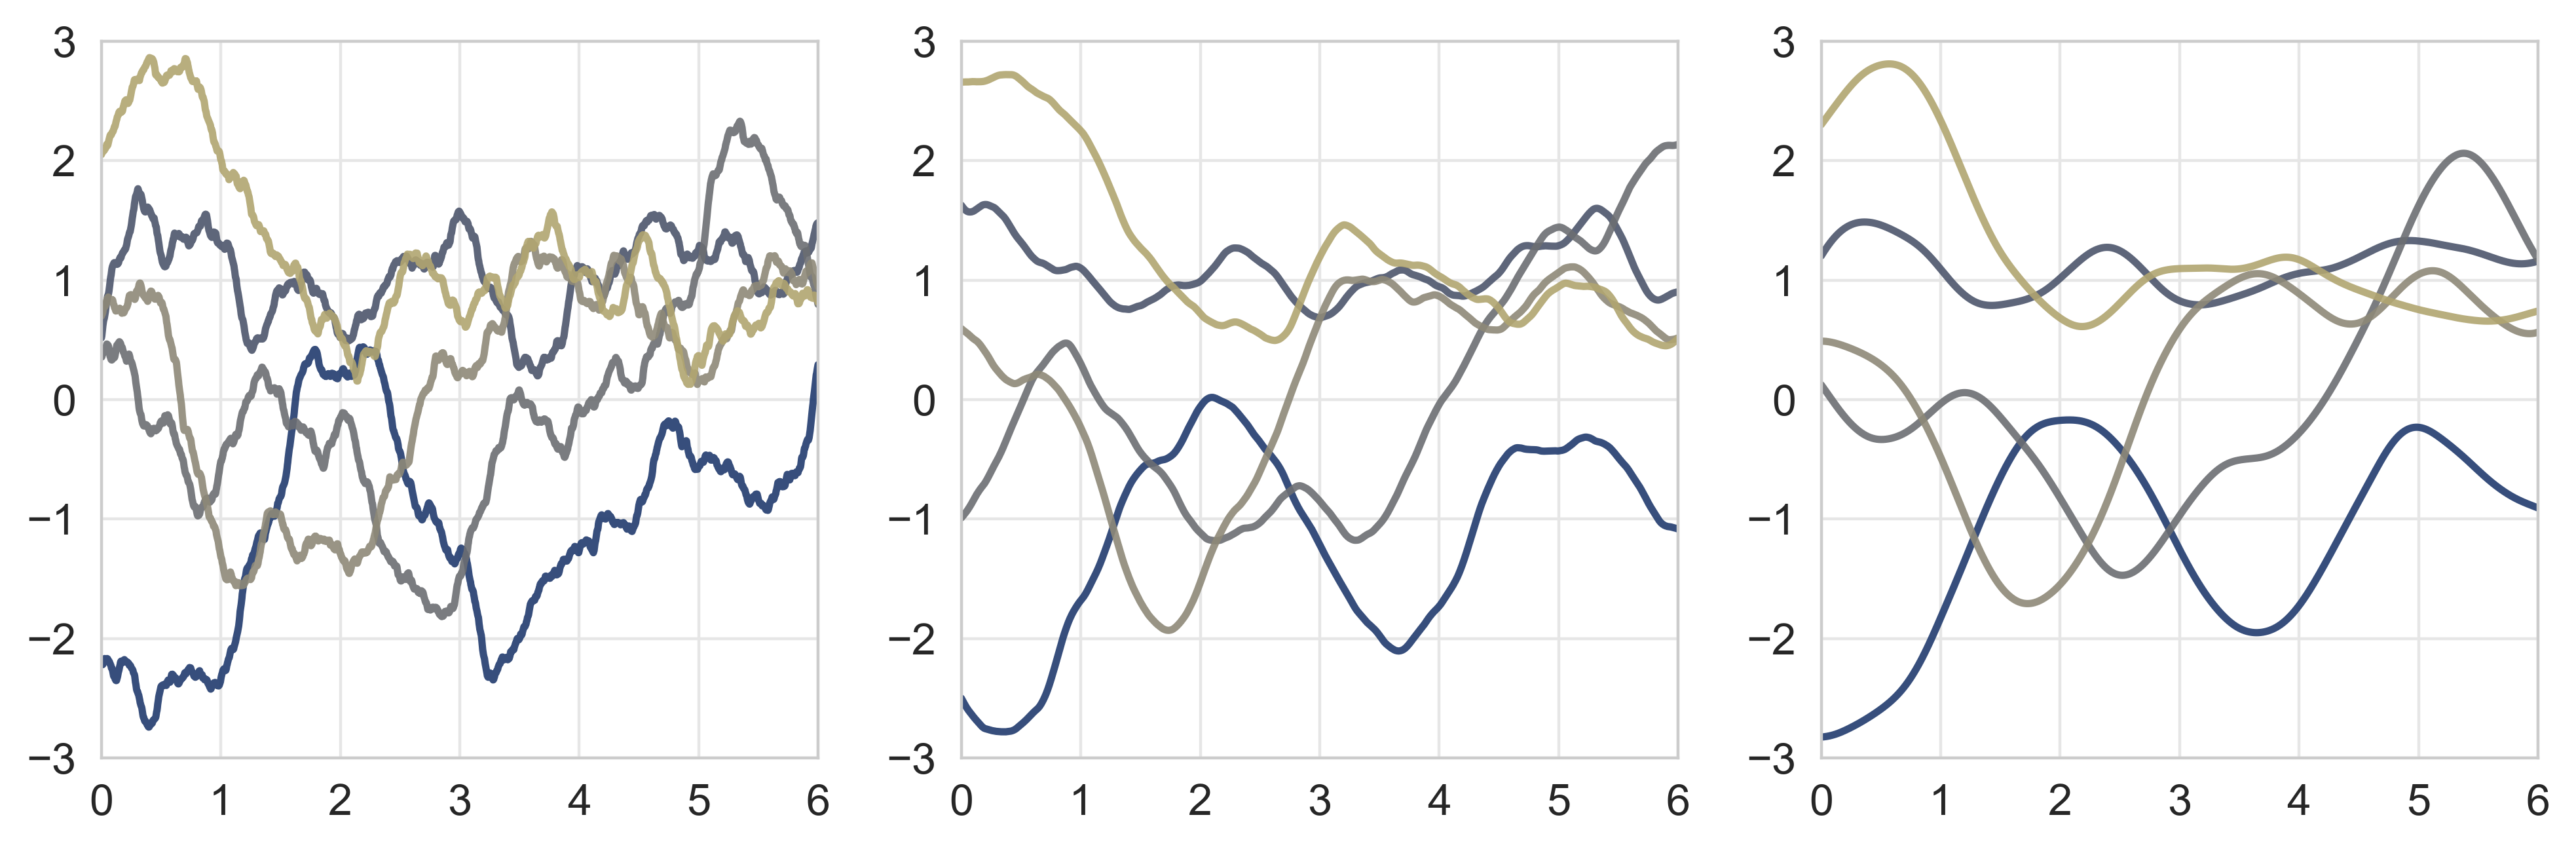
\includegraphics[width=1\textwidth,height=\textheight]{figures/matern_simulation_1d.png}

}

\caption{\label{fig-matern-1d}Five random simulations from a Gaussian
Process defined on \(\mathbb{R}\) with zero mean and Matérn-\(\nu\)
covariance function, with \(\nu=1\) (left), \(\nu=2\) (middle), and
\(\nu=4\) (right), showing that higher values of \(\nu\) produce
smoother curves.}

\end{figure}%

\begin{figure}

\centering{

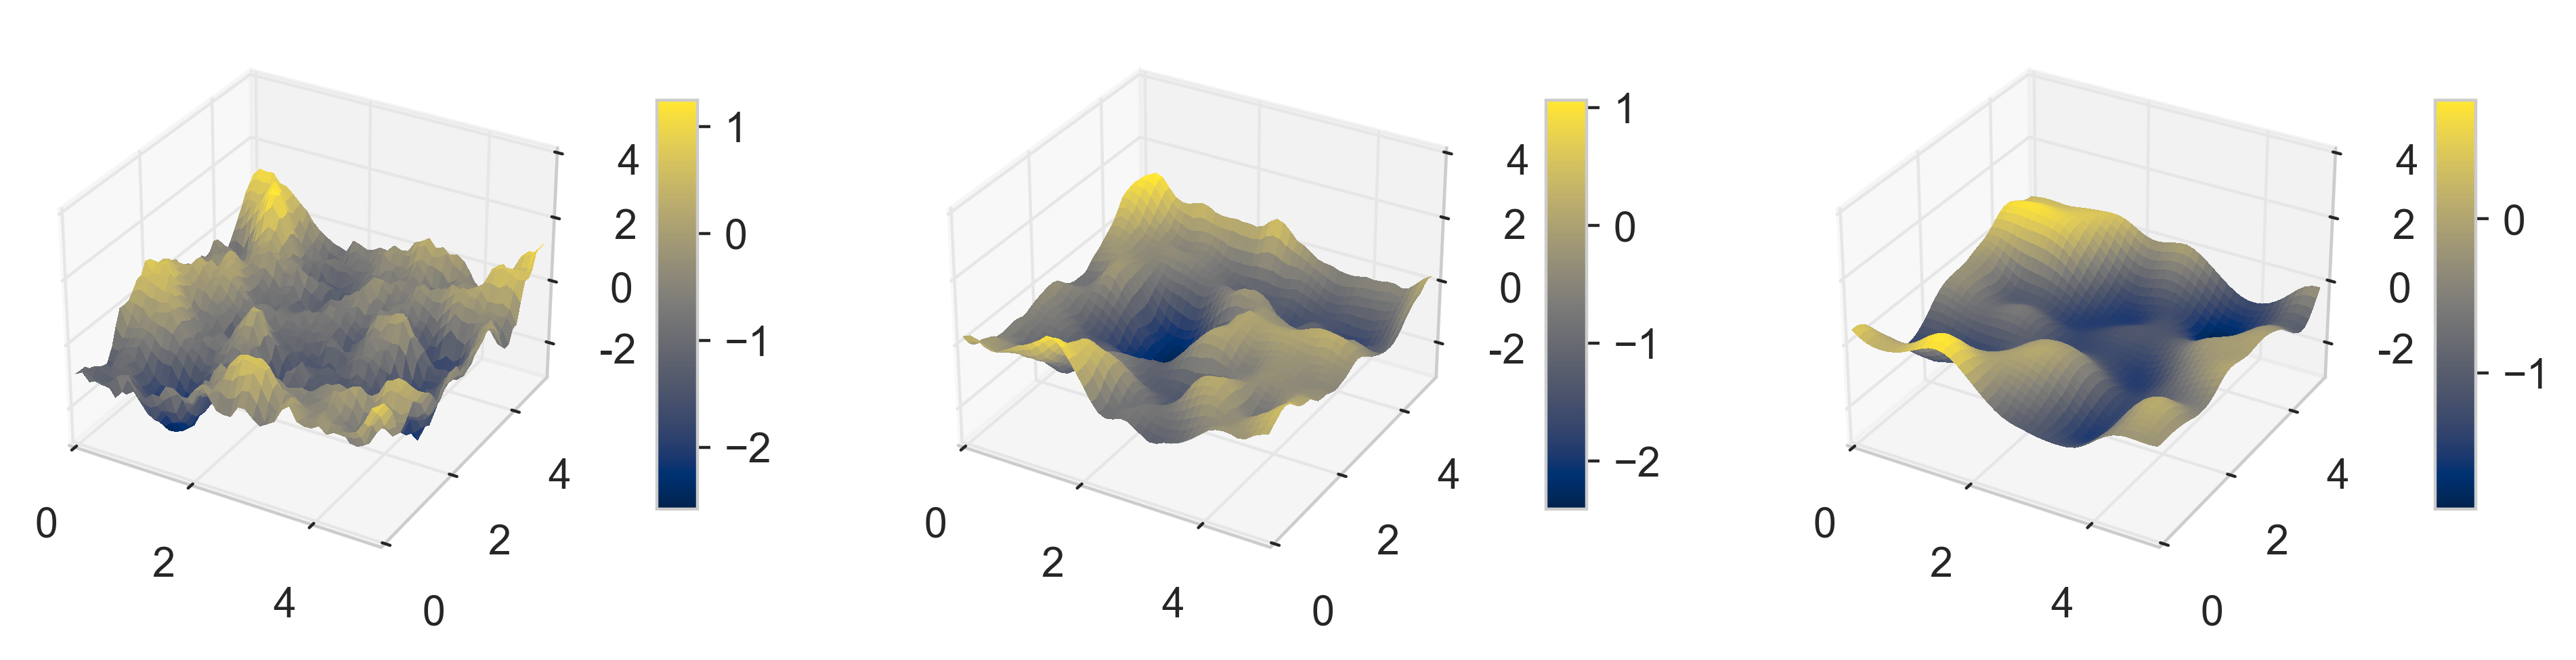
\includegraphics[width=1\textwidth,height=\textheight]{figures/matern_simulation_2d.png}

}

\caption{\label{fig-matern-2d}One random simulation from a Gaussian
Process defined on \(\mathbb{R}^2\) with zero mean and Matérn-\(\nu\)
covariance function, with \(\nu=1\) (left), \(\nu=2\) (middle), and
\(\nu=4\) (right), showing that higher values of \(\nu\) produce
smoother surfaces.}

\end{figure}%

In view of these results, the parameter \(\nu\) is suggested as a
measure of the smoothness of the PP index function by fitting a Gaussian
process prior with Matérn covariance on a dataset generated by random
evaluations of the index function, as done at the initialization stage
of the jellyfish search optimization. There exist several R packages,
such as \texttt{GpGp} (Guinness, Katzfuss, and Fahmy 2021) or
\texttt{ExaGeoStatR} (Abdulah et al. 2023), to fit the hyperparameters
of a GP covariance function on data, which is usually done by maximum
likelihood estimation. In this project, the \texttt{GpGp} package is
used.

\begin{defn}
Let $\mathbf{A}=[A_1, \ldots, A_N] \in (\mathbf{R}^{p \times d})^N$ be d-dimensional projection bases, let $\mathbf{y}=[f(XA_1),\ldots,f(XA_N)]$ be the corresponding PP index values, and let $\mathbf{K}=[K_\theta(A_{i},A_{j})]_{1\leq i,j\leq N}\in\mathbb{R}^{N\times N}$ be the Matérn covariance matrix evaluated at the input bases, where the vector $\theta$ contains all the parameters of the multivariate Matérn covariance function $K$ (smoothness, outputscale, lengthscales). The log-likelihood of the parameters $\theta$ is defined by 
\begin{equation}
\mathcal{L}(\theta)=\log p(\mathbf{y}\left|\mathbf{A},\theta\right.)=-\frac{1}{2}\mathbf{y}^{\top}(\mathbf{K}+\sigma^{2}\mathbf{I})^{-1}\mathbf{y}-\frac{1}{2}\mathrm{\log}(\det(\mathbf{K}+\sigma^{2}\mathbf{I}))-\frac{N}{2}\log(2\pi)\, \label{eq:gp_log_likelihood}
\end{equation}
where the nugget parameter $\sigma$ is the standard deviation of the intrinsic noise of the Gaussian process.
The optimal parameters (including smoothness) are obtained by maximum log-likelihood
\begin{equation}
\theta^* = \underset{\theta}{\max}\mathcal{L}(\theta)
\end{equation}
The resulting optimal smoothness parameter $\nu$ is chosen as our smoothness metric.
\end{defn}

The value of the optimal smoothness parameter \(\nu>0\) can be naturally
interpreted as follows: the higher \(\nu\), the smoother the index
function.

\subsection{Squintability}\label{sec-squintability}

Here the formal definition of projection distance and squint angle are
given, before the definition of squintability. Two approaches to compute
this metric numerically, are described.

\begin{defn}[projection distance]\label{def:proj-dist}
Recall that $A \in \mathbf{R}^{p \times d}$ is a $d$-dimensional orthonormal matrix. Let $A^*$ be the optimal matrix that achieves the maximum index value for a given data. The projection distance $d(A, A^*)$ between $A$ 
and $A^*$ is defined as 
$d(A, A^*) = \lVert AA^\prime - A^*A^{*\prime}\  \rVert _F$
where $\lVert . \rVert _F$ denotes the Frobenius norm, given by
$\lVert M \rVert _F = \sqrt{\sum_{ij} M_{ij}^2}$. 
\end{defn}

\begin{defn}[squint angle]\label{def:squint-angle}
Let $A$ and $B$ be two $d$-dimensional orthonormal matrices in $\mathbb{R}^p$. The squint angle $\theta$ between the subspace spanned by $A$ and $B$ is defined as the smallest principal angle between these subspaces: $\theta = \min_{i \in \{1, \cdots, d\}} \arccos(\tau_i)$, where $\tau_i$ are the singular values of the matrix $M = A^T B$ obtained from its singular value decomposition.

\end{defn}

Squintability can be defined as how the index value \(f(XA)\) changes
with respect to the projection distance \(d(A, A^*)\), over the course
of the JSO:

\begin{defn}[squintability]\label{def:squintability}
Let $g: \mathbb{R} \mapsto  \mathbb{R}$ be a decreasing function that maps the projection distance $d(A, A^*)$ to the index value $f(XA)$, such that $g(d(A, A^*)) = f(XA)$. For brevity, denote $g(d)$ as $g(d(A, A^*))$. The squintability of an index function $f(XA)$ is defined as 

\begin{equation}
\varsigma(f) = -c \times \max_{d} g'(d) \times \arg \max_{d} g'(d)
\label{eq-squintability}
\end{equation}

where $c$ is a constant scaling factor, $-\max_d g'(d)$ represents the 
largest gradient of $-g$ and $\arg \max_{d} g'(d)$ represents the projection distance at which this largest gradient is attained.

\end{defn}

It is expected that these two values should be both high in the case of
high squintability (fast increase in \(f\) early on), and both low in
the case of low squintability (any substantial increase in \(f\) happens
very late, close to the optimal angle). This suggests that their product
\eqref{eq-squintability} should provide a sensible measure of
squintability. The multiplicative constant \(4\), which can be deemed
arbitrary, does not change the interpretation of the squintability
metric \(\varsigma\); it is here to adjust the range of values of
\(\varsigma\) and simplify the explicit formula for \(\varsigma\)
obtained later on.

From the definition, the following proposition can be derived:

\begin{prop}\label{prop:convex-concave}
Let $g_1(d)$ be a convex decreasing function and $g_2(d)$ be a concave decreasing function both defined on [0, 1] where $d \in [0, D]$. Let $d_1 := \underset{d}{\arg \max} |g_1'(d)|$ and $d_2 := \underset{d}{\arg \max} |g_2'(d)|$.

$$\varsigma(g_1) < \varsigma(g_2)$$

For a convex function, $g_1'(d) < 0 \; \forall d$ and is non-decreasing. For a concave function, $g_2'(d) < 0 \; \forall d$ and is non-increasing. As such, it follows that $d_1 < d_2$.

Suppose both functions achieve the same maximum gradient $-g_{\max}$, i.e., $\max g'_1(d_1) = \max g'_2(d_2) = -g_{\max}$,

$$
\varsigma(g_1(d_1)) = -c  \max g'_1(d_1)  d_1 = -c  (-g_{\max}) d_1 \leq -c  (-g_{\max}) d_2 = -c \max g'_2(d_2)  d_2 = \varsigma(g_2(d_2))
$$

\end{prop}

From Tukey and Tukey (1981) and Laa and Cook (2020), a large squint
angle implies that the objective function value is close to optimal even
when the perfect view to see the structure is far away. A small squint
angle means that the PP index value improves substantially only when the
perfect view is close by. As such, low squintability implies rapid
improvement in the index value when near the perfect view. For PP, a
small squint angle is considered to be undesirable because it means that
the optimiser needs to be very close to be able to ``see'' the optima.
Thus, it could be difficult for the optimiser to find the optima.

It is expected that for a PP index with high squint angle, the
optimization (\ref{eq-optimization}) should make substantial progress
early on. Conversely, for a PP index with low squint angle, it might
take a long while for the optimization to make substantial progress, as
the candidate projections would need to be very close to the optimal one
for the structure of the index function to be visible enough to be
amenable to efficient optimization. This observation suggests that the
extreme values of \(f'\) (the ones for which \(f''=0\), assuming that
\(f\) is twice differentiable), and the projection distances for which
these values are attained, are crucial in the mathematical definition of
squintability.

To compute the squintability metric \eqref{eq-squintability} in
practice, several approaches are possible. The first one is to propose a
parametric model for \(f\), and use it to obtain an explicit formula for
\(\varsigma\). Numerical experiments suggest a scaled sigmoid shape as
described below. Define

\begin{equation}\phantomsection\label{eq-logistic}{
\ell(x):=\frac{1}{1+\exp(\theta_{3}(x-\theta_{2}))}\ ,
}\end{equation}

which is a decreasing logistic function depending on two parameters
\(\theta_2\) and \(\theta_3\), such that
\(\ell(\theta_{2})=\frac{1}{2}\). Then, define

\begin{equation}\phantomsection\label{eq-parametric}{
f(x)=(\theta_{1}-\theta_{4})\frac{\ell(x)-\ell(x_{\max})}{\ell(0)-\ell(x_{\max})}+\theta_{4}\ ,
}\end{equation}

which depends on three additional parameters, \(\theta_1\),
\(\theta_2\), and \(x_{\max}\), such that \(f(0)=\theta_1\) and
\(f(x_{\max})=\theta_4\). Under the parametric model
(\ref{eq-parametric}), the squintability metric \eqref{eq-squintability}
can be shown to be equal to

\begin{equation}\phantomsection\label{eq-squintability-parametric}{
\varsigma=\frac{(\theta_{1}-\theta_{4})\theta_{2}\theta_{3}}{\ell(0)-\ell(x_{\max})}\ .
}\end{equation}

In practice, the parameters of this model (\ref{eq-parametric}) can be
estimated numerically, for example by non-linear least squares, and then
used to evaluate \(\varsigma\) as in equation
(\ref{eq-squintability-parametric}).

Alternatively, one can estimate \eqref{eq-squintability} in a
nonparametric way, for example by fitting \(f\) using kernel regression,
then numerically estimate the angle at which \(-f'\) attains its highest
value.

\section{The jellyfish optimiser}\label{sec-JSO}

JSO mimics the natural movements of jellyfish, which include passive and
active motions driven by ocean currents and their swimming patterns,
respectively. In the context of optimization, these movements are
abstracted to explore the search space, aiming to balance exploration
(searching new areas) and exploitation (focusing on promising areas).
The algorithm aims to find the optimal solution by adapting the
behaviour of jellyfish to navigate towards the best solution over
iterations (Chou and Truong 2021).

To solve the optimisation problem embedded in the PP guided tour, a
starting projection, an index function, the number of jellyfish, and the
maximum number of trials (tries) are provided as input. Then, the
current projection is evaluated by the index function. The projection is
then moved in a direction determined by a random factor, influenced by
how far along we are in the optimisation process. Occasionally,
completely new directions may be taken like a jellyfish might with ocean
currents. A new projection is accepted if it is an improvement compared
to the current one, rejected otherwise. This process continues and
iteratively improves the projection, until the pre-specified maximum
number of trials is reached.

\begin{tcolorbox}[enhanced jigsaw, rightrule=.15mm, breakable, toprule=.15mm, bottomtitle=1mm, colframe=quarto-callout-note-color-frame, arc=.35mm, titlerule=0mm, coltitle=black, bottomrule=.15mm, opacityback=0, opacitybacktitle=0.6, title={Algorithm: Jellyfish Optimizer Pseudo Code}, colbacktitle=quarto-callout-note-color!10!white, left=2mm, colback=white, leftrule=.75mm, toptitle=1mm]

\textbf{Input}: \texttt{current\_projections}, \texttt{index\_function},
\texttt{trial\_id}, \texttt{max\_trial}

\textbf{Output}: \texttt{optimised\_projection}

\textbf{Initialize} \texttt{current\_best} as the projection with the
best index value from \texttt{current\_projections}, and
\texttt{current\_idx} as the array of index values for each projection
in \texttt{current\_projections}

\textbf{for} each \texttt{trial\_id} in 1 to \texttt{max\_tries}
\textbf{do}

\begin{quote}
Calculate the time control value, \(c_t\), based on
\texttt{current\_idx} and \texttt{max\_trial}
\end{quote}

\begin{quote}
\textbf{if} \(c_t\) is greater than or equal to \(0.5\) \textbf{then}

\begin{quote}
Define trend based on the \texttt{current\_best} and
\texttt{current\_projections}
\end{quote}

\begin{quote}
Update each projection towards the trend using a random factor and
orthonormalisation
\end{quote}

\textbf{else}

\begin{quote}
\textbf{if} a random number is greater than \(1 - c_t\) \textbf{then}

\begin{quote}
Slightly adjust each projection with a small random factor (passive)
\end{quote}

\textbf{else}

\begin{quote}
For each projection, compare with a random jellyfish and adjust towards
or away from it (active)
\end{quote}
\end{quote}

Update the orientation of each projection to maintain consistency

Evaluate the new projections using the index function
\end{quote}

\begin{quote}
\textbf{if} any new projection is worse than the current, revert to the
\texttt{current\_projections} for that case

\begin{quote}
Determine the projection with the best index value as the new
\texttt{current\_best}
\end{quote}
\end{quote}

\begin{quote}
\textbf{if} \texttt{trial\_id} \(\ge\) \texttt{max\_trial}, print the
last best projection \textbf{exit}
\end{quote}

\textbf{return} the set of projections with the updated
\texttt{current\_best} as the \texttt{optimised\_projection}

\end{tcolorbox}

The JSO implementation involves several key parameters that control its
search process in optimization problems. These parameters are designed
to guide the exploration and exploitation phases of the algorithm. While
the specific implementation details can vary depending on the version of
the algorithm or its application, the focus is on two main parameters
that are most relevant to our application: the number of jellyfish and
the maximum number of tries.

\section{Simulation study}\label{sec-sim-deets}

The JSO performance is compared with an existing optimiser, Creeping
Random Search (CRS) (Zhang et al. 2021; Laa and Cook 2020) used in the
PP guided tour to explore JSO's behaviour under different
hyper-parameter and data dimension combinations. The second simulation
studies the effect of index properties (smoothness and squintability),
along with JSO hyper-parameters, and data dimension, on the success rate
of the JSO performance. This section describes the simulation details,
with the results deferred to Section~\ref{sec-sim-res}.

\subsection{Performance of JSO relative to CRS}\label{sec-app-1}

The performance of JSO is investigated both in comparison to the
existing optimizer, CRS, and across various hyper-parameter values. The
performance is measured by the success rate, defined as the proportion
of simulations that achieves a final index value within 0.05 of the best
index value found among all 50 simulations (see
Figure~\ref{fig-success-rate} for an illustration). This comparison is
based on projection pursuit to find the pipe shape investigated by Laa
and Cook (2020) using the \texttt{holes} index.

Fifty simulations are conducted with both JSO and CRS, in four different
data dimensions (\(d = 6, 8, 10, 12\)). JSO uses 100 jellyfishes with a
maximum of 100 tries, while the CRS allows a maximum of 1000 samples at
each iteration before the algorithm terminates. The different numbers
account for the multiple paths of JSO to enable fairer comparison with
CRS. The results of the simulation are collected using the data
structure proposed in Zhang et al. (2021) for assessing JSO, where the
design parameters are stored along with index value, projection basis,
random seed, and computation time.

Fifty additional simulations are conducted for each hyper-parameter
combination to analyze how they affect the JSO success rate. This
includes variations in the number of jellyfish (20, 50, and 100) and the
maximum number of tries (50 and 100).

\begin{figure}

\centering{

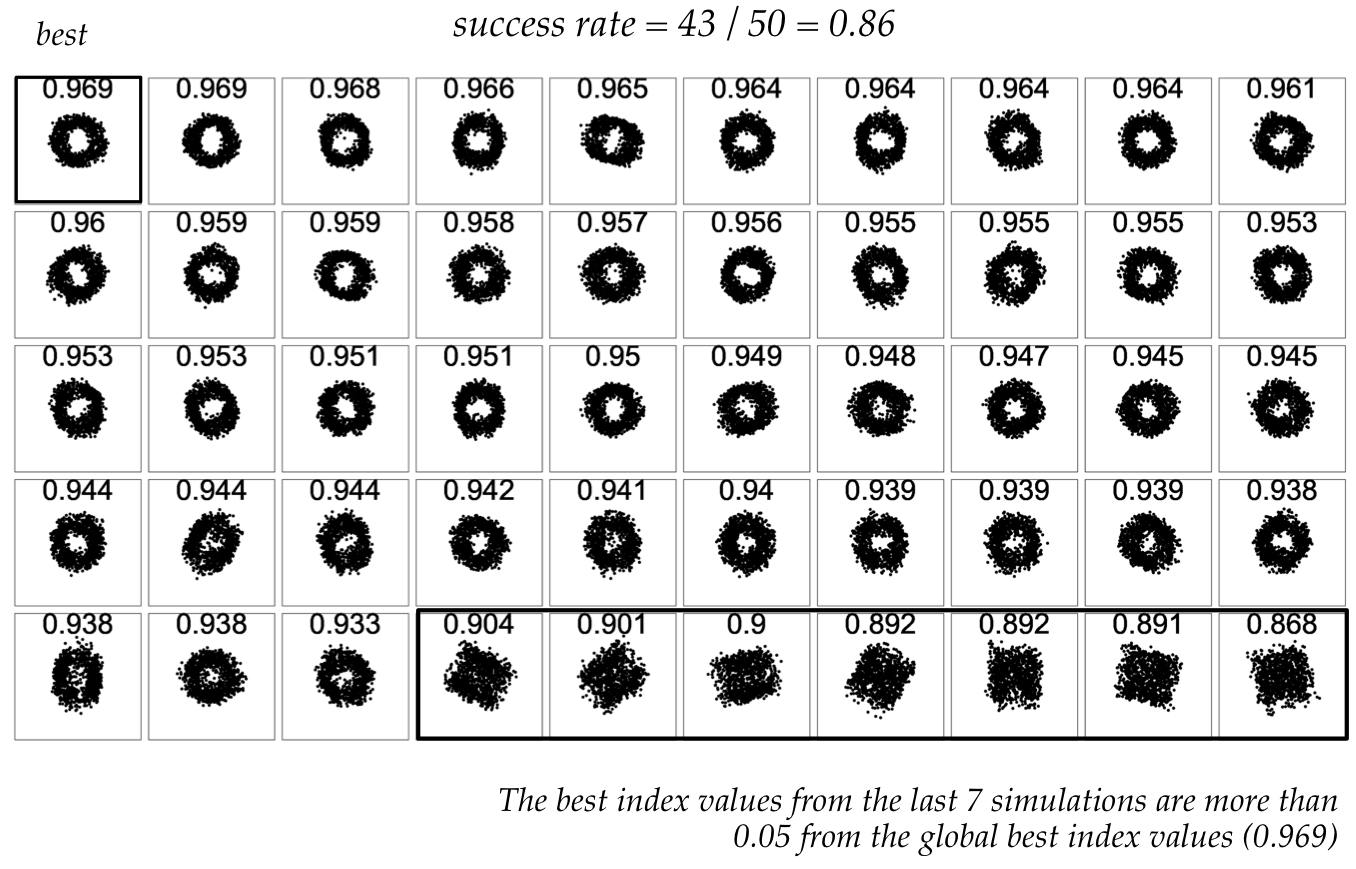
\includegraphics[width=4.52in,height=\textheight]{figures/success-rate.png}

}

\caption{\label{fig-success-rate}Illustration of success rate
calculation: Final projections based on projection pursuit to find the
pipe shape in 8D data using the holes index, optimised by CRS, in 50
simulations. The 50 final projections are sorted by their index values.
The highest index value found across all simulations is 0.969. Out of
the 50 simulations, 43 achieved an index value within 0.05 of the best,
resulting in a success rate of 0.86 (43/50).}

\end{figure}%

\subsection{Factors affecting JSO success rate: index properties and
jellyfish hyper-parameters}\label{sec-app-2}

To assess JSO's performance across various scenarios, two different data
shapes, pipe and a sine wave, are investigated in 6D and 8D spaces using
six different PP indexes: \texttt{dcor2d\_2}, \texttt{loess2d},
\texttt{MIC}, \texttt{TIC}, \texttt{spline}, and \texttt{stringy}, with
varied JSO hyper-parameters. A total of 52 combinations result,
comprising of 24 computed on the pipe data and 28 on the sine-wave data.
Again, JSO is run 50 times to calculate the success rate for each
projection pursuit.

Smoothness and squintability are computed following the procedures
outlined in Section~\ref{sec-smoothness} and
Section~\ref{sec-squintability} and as illustrated in
Figure~\ref{fig-smoothness} and Figure~\ref{fig-squintability}. To
compute smoothness, 300 random bases are simulated. Index values and
projection distance (to the optimal basis) are calculated for each
random basis before fitting the Gaussian process model to obtain the
smoothness measure for the index.

To compute squintability, 50 random bases are sampled and interpolated
to the optimal basis with a step size of 0.005. Index values and
projection distances are calculated for these interpolated bases and the
index values are averaged with a bin width of 0.005. A four-parameter
scaled logistic function is fitted to the index values against
projection distances, estimated by non-linear least squares. The
squintability measure is then calculated as
(\ref{eq-squintability-parametric}).

To construct a relationship among success rate, index properties
(smoothness and squintability), and jellyfish hyper-parameters, a
generalised linear model is fitted using a binomial family and a logit
link function. The data is pre-processed by 1) scaling the JSO
hyper-parameters by a factor of 10 for interpretation, 2) creating a new
binary variable \texttt{long\_time} to indicate cases with an average
run time over 30 seconds, and 3) re-coding the success rate for the
\texttt{stringy} index as 0, because none of the 50 simulations
correctly identified the sine-wave shape.

\begin{figure}

\centering{

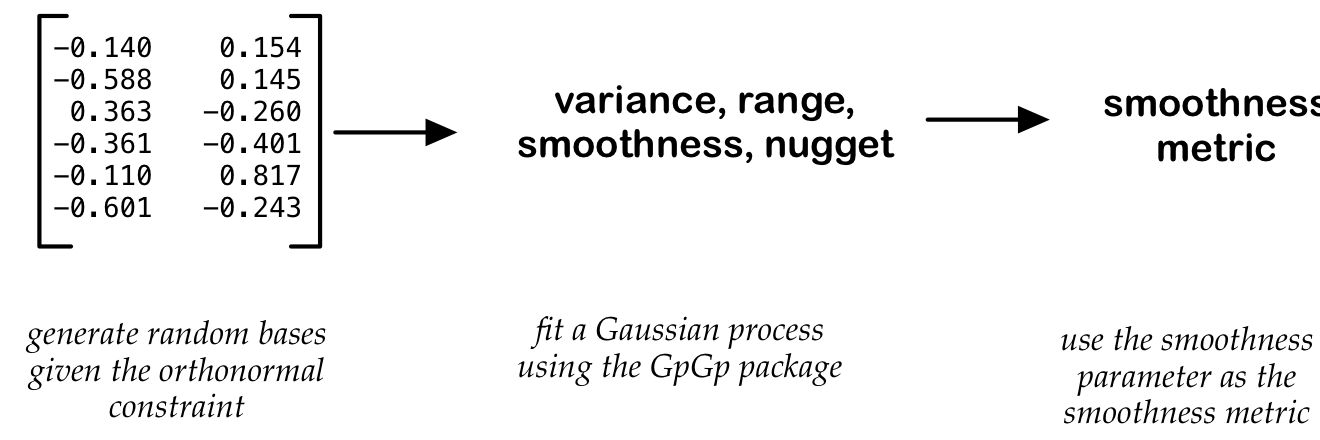
\includegraphics[width=1\textwidth,height=\textheight]{figures/smoothness.png}

}

\caption{\label{fig-smoothness}Illustration of steps to calculate
smoothness. For a given projection pursuit problem defined by the shape
to find, data dimension and the index function, 1) sample random bases
given the orthonormality contraint, 2) calculate the projection distance
and the index value for each random basis, and 3) fit a Gaussian process
model of index values against projection distances to obtain the
smoothness measure.}

\end{figure}%

\begin{figure}

\centering{

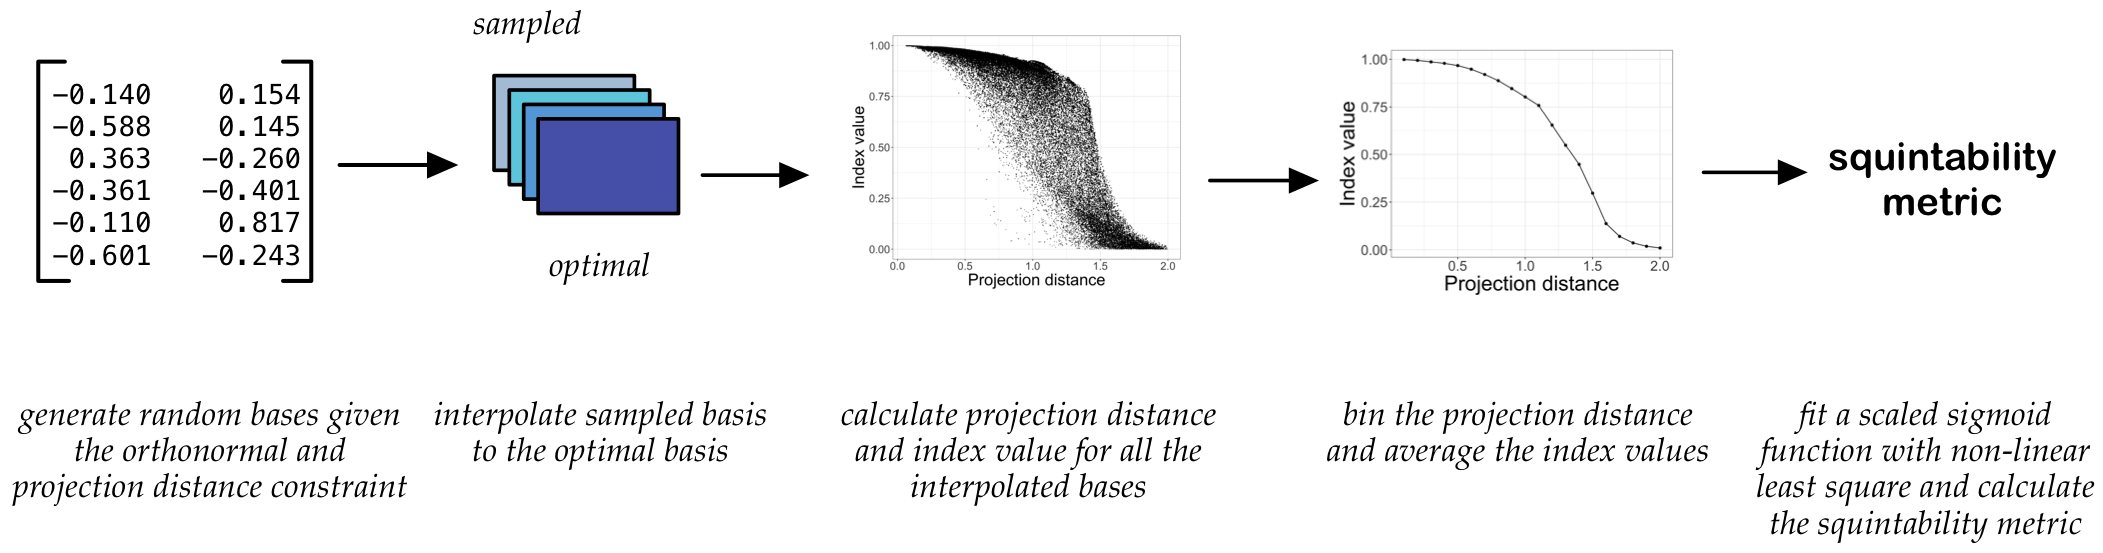
\includegraphics[width=1\textwidth,height=\textheight]{figures/squintability.png}

}

\caption{\label{fig-squintability}Illustration of steps to calculate
squintability. For a given projection pursuit problem defined by the
shape to find, data dimension and the index function, 1) sample random
bases given the orthonormality and projection distance contraint, 2)
interpolate the sampled bases to the optimal basis and calculate the
projection distance and the index value for each interpolated basis. 3)
bin the index values by projection distances to obtain the average index
value for each bin, 4) fit the scaled sigmoid function in equation
\eqref{eq-squintability} to the binned index values against projection
distances using non-linear least square, 5) calculate the squintability
measure using equation (\ref{eq-squintability-parametric}) with
parameters estimated from the model.}

\end{figure}%

\section{Results}\label{sec-sim-res}

The results from the first simulation described in
Section~\ref{sec-sim-deets} are analysed based on the final projections
across two optimisers (JSO and CRS) and the success rate across JSO
hyper-parameters. In the second simulation, smoothness and squintability
are calculated across a collection of pipe-finding and sine-wave finding
problems to construct the relationship between success rate, JSO
hyper-parameters, and index properties.

The final projections found by the two optimisers (JSO and CRS) are
presented in Figure~\ref{fig-proj}, broken down by 10th quantile,
faceted by the data dimensions. In the 6-dimensional data scenario, JSO
consistently identifies a clear pipe shape. The CRS also finds the pipe
shape but with a wide rim, suggesting a further polish search may be
required. With increasing dimensions, JSO may not always identify the
pipe shape due to random sampling, but it still finds the pipe shape in
over 50\% of cases. Compared to CRS, JSO achieves higher index values
and clearer pipe shapes across all quantiles in data of 8, 10, 12
dimensions, suggesting its advantage in exploring high-dimensional
spaces.

The success rate calculated at each hyper-parameter combination (number
of jellyfish and the maximum number of tries) is presented in
Figure~\ref{fig-proportion}. The uncertainty is quantified through 500
bootstrap replicates for each case. As the number of jellyfish and
maximum tries increase, the success rate also increases. For simpler
problems (6 dimensions), small parameter values (20 jellyfishes and a
maximum of 50 tries) can already achieve a high success rate. However,
larger parameter values (i.e.~100 jellyfishes and a maximum of 100
tries) are necessary for higher-dimensional problems (8, 10, and 12
dimensions). Increasing both parameters enhances the performance of JSO,
but it also extends the computational time required for the
optimisation, which can be computationally intensive when evaluating the
index function (such as scagnostic indexes) multiple times across
numerous iterations.

\begin{figure}

\centering{

\includegraphics{jso_files/figure-pdf/fig-proj-1.pdf}

}

\caption{\label{fig-proj}Projections found by the JSO and CRS at each
10th quantile across 50 simulations. The projection pursuit problem is
to find the pipe shape using the holes index in the 6, 8, 10, and
12-dimensional spaces. The JSO uses 100 jellyfishes and a maximum number
of tries of 100. The CRS uses a maximum of 1000 tries in each step of
random sampling step before the algorithm terminates. In the 6-D data
space, JSO always finds a clear pipe shape while the CRS also finds the
pipe shape but with a wide rim. At higher data dimensions, JSO finds a
higher index value and a clearer pipe shape across all the quantiles
than the CRS}

\end{figure}%

\begin{figure}

\centering{

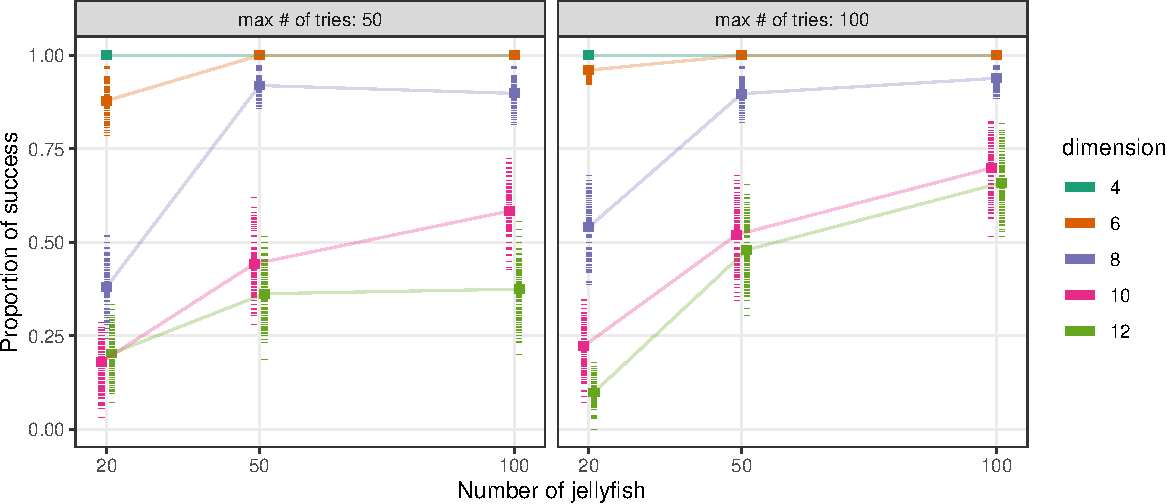
\includegraphics{jso_files/figure-pdf/fig-proportion-1.pdf}

}

\caption{\label{fig-proportion}The proportion of simulations that reach
near-optimal index values in the pipe-finding problem using the holes
index. The proportion is calculated based on the number of simulations,
out of 50, that achieve an index value within 0.05 of the
best-performing simulation. To quantify uncertainty, Bootstrap samples
with 500 are generated. The thin lines represent the proportion for each
of the 500 bootstrap replicates, while the thicker lines represent the
mean of these bootstrap samples, connnected by lines. As the
dimensionality increases, the proportion of simulations reaching the
optimal index value increases.}

\end{figure}%

The index properties, including smoothness and squintability, offer
numerical metrics to characterise the complexity of projection pursuit
optimisation problems. Table~\ref{tbl-smoothness-squintability} presents
the parameters for calculating both metrics estimated from the Gaussian
process (variance, range, smooth, and nugget) and the scaled logistic
function (\(\theta_1\) to \(\theta_4\)) for each case considered in the
simulation. The column ``smooth'' is used as the smoothness metric and
the column ``squint'' is calculated as equation
(\ref{eq-squintability-parametric}) as the squintability metric.
Table~\ref{tbl-mod-output} presents the results of fitting a generalised
linear model with a binomial family and a logit link function. The model
suggests that JSO success rate is positively associated with the two
hyper-parameters, as well as with the index properties: smoothness and
squintability. Specifically, using 10 more jellyfish and 10 more tries
increases the odd ratio of success by 24.11\% and 11.93\%, respectively.
However, being flagged with long runtime and an increase of data
dimension reduce the success rate by 41.72\% and 53.36\%, respectively.
The variable \texttt{squintability} and \texttt{dimension} are
significant, suggesting their importance relative to JSO
hyper-parameters in the optimisation success.

\begin{table}

\caption{\label{tbl-smoothness-squintability}Parameters estimated from
the Gaussian process (outputscale \(\eta\), lengthscale \(\ell\),
smoothness \(\nu\), and nugget \(\sigma\)) and scaled logistic function
(\(\theta_1\) to \(\theta_4\) and \(\varsigma\)) for the pipe-finding
and sine-wave finding problems. The columns \(\nu\) and \(\varsigma\)
represent the smoothness and squintability measures respectively.}

\centering{

\centering\begingroup\fontsize{10}{12}\selectfont

\begin{tabular}{|>{}lcc>{}c|ccc>{}c|cccc>{}c|}
\toprule
  & shape & index & d & $\eta$ & $\ell$ & $\nu$ & $\sigma$ & $\theta_1$ & $\theta_2$ & $\theta_3$ & $\theta_4$ & $\varsigma$\\
\midrule
1 & pipe & holes & 6 & 0.04 & 0.37 & 2.36 & 0.22 & 1.02 & 0.86 & 3.37 & 0.02 & 3.05\\
2 & pipe & holes & 8 & 0.01 & 0.18 & 2.19 & 0.82 & 1.01 & 0.87 & 3.26 & 0.03 & 2.96\\
3 & pipe & holes & 10 & 0.01 & 0.11 & 2.19 & 3.03 & 1.02 & 0.88 & 3.15 & 0.02 & 2.95\\
4 & pipe & holes & 12 & 0.01 & 0.15 & 2.29 & 1.58 & 1.01 & 0.88 & 3.34 & 0.00 & 3.12\\
5 & sine & MIC & 6 & 0.13 & 0.09 & 2.46 & 0.08 & 0.89 & 0.57 & 1.62 & -0.02 & 1.26\\
6 & sine & MIC & 8 & 0.13 & 0.08 & 2.64 & 0.08 & 0.93 & 0.33 & 1.31 & -0.03 & 0.77\\
7 & sine & TIC & 6 & 0.35 & 0.11 & 2.44 & 0.09 & 0.95 & 0.54 & 1.72 & -0.03 & 1.32\\
8 & sine & TIC & 8 & 0.35 & 0.10 & 2.47 & 0.09 & 0.95 & 0.56 & 1.72 & -0.03 & 1.37\\
9 & sine & dcor & 6 & 0.18 & 0.17 & 2.66 & 0.11 & 0.95 & 1.04 & 2.74 & -0.02 & 2.95\\
10 & sine & loess & 6 & 0.28 & 0.34 & 1.99 & 0.31 & 1.02 & 1.04 & 2.65 & 0.08 & 2.76\\
11 & sine & splines & 6 & 0.20 & 0.24 & 2.54 & 0.10 & 1.01 & 1.05 & 2.73 & -0.01 & 3.12\\
12 & sine & stringy & 6 & 0.00 & 0.01 & 1.54 & 38.17 & 1.05 & 0.01 & 254.73 & 0.05 & 2.96\\
\bottomrule
\end{tabular}
\endgroup{}

}

\end{table}%

\begin{table}

\caption{\label{tbl-mod-output}Model estimates of proportion of jellyfish success on index properties and jellyfish hyper-parameters from the generalised linear model with a binomial family and a logit link function.The variable smoothness, squintability, number of jellyfish and maximum number of tries are positively associated with JSO success rate while data dimension and being flagged as long runtime are negatively associated with the success rate. The variable squintability and dimension are significant, suggesting their importance relative to jellyfish hyper-parameters in the optimisation success. }

\centering{

[H] \centering 
   
   
\begin{tabular}{@{\extracolsep{5pt}}lc} 
\\[-1.8ex]\hline 
\hline \\[-1.8ex] 
 & \multicolumn{1}{c}{\textit{Dependent variable:}} \\ 
\cline{2-2} 
\\[-1.8ex] & proportion \\ 
\hline \\[-1.8ex] 
 Smoothness & 1.195 \\ 
  & (1.915) \\ 
  & \\ 
 Squintability & 2.060$^{***}$ \\ 
  & (0.684) \\ 
  & \\ 
 Dimension & $-$0.628$^{**}$ \\ 
  & (0.255) \\ 
  & \\ 
 Long runtime & $-$0.874 \\ 
  & (1.286) \\ 
  & \\ 
 Number of jellyfish & 0.216$^{*}$ \\ 
  & (0.127) \\ 
  & \\ 
 Maximum number of tries & 0.113 \\ 
  & (0.150) \\ 
  & \\ 
 Constant & $-$4.523 \\ 
  & (5.332) \\ 
  & \\ 
\hline \\[-1.8ex] 
Observations & 52 \\ 
Log Likelihood & $-$18.224 \\ 
Akaike Inf. Crit. & 50.447 \\ 
\hline 
\hline \\[-1.8ex] 
\textit{Note:}  & \multicolumn{1}{r}{$^{*}$p$<$0.1; $^{**}$p$<$0.05; $^{***}$p$<$0.01} \\ 
\end{tabular} 

}

\end{table}%

\section{Practicalities}\label{sec-discussion}

The simulation study demonstrated the that these metrics can be used to
assess a PP index, and compare optimisers. Here we explain how they can
be used for new index and optimiser development. Using the JSO optimiser
for GTPP requires a change in user behaviour. For all the existing
optimisers a single optimisation path is followed. The JSO has multiple
optimisation paths, and needs additional tools to incorporate into the
PPGT, as explained here.

\subsection{Using the JSO in a PPGT}\label{using-the-jso-in-a-ppgt}

To use JSO for PPGT in the \texttt{tourr} package, specify
\texttt{search\_f\ =\ search\_jellyfish} in the guided tour. Since
multiple tour paths are generated by the jellyfish, the animation
function \texttt{animate\_*()} will not render the tour path for JSO. To
visualise path visited by each individual jellyfish, assign the
animation to an object (\texttt{res\ \textless{}-\ animate\_xy(...)}).
This will save the bases visited by the optimiser, along with relevant
metadata, as a tibble data object (see Zhang et al. (2021) for more
details on the data object). The bases visited for individual jellyfish
can then be extracted and viewed using the \texttt{planned\_tour()}
function.

\subsection{Computing the metrics for your new
index}\label{computing-the-metrics-for-your-new-index}

The \texttt{ferrn} package (Zhang et al. 2021) provides functionality
for computing the smoothness and squintability metrics. Both cases
require sampling random bases using the \texttt{sample\_bases()}
function, followed by calculating the specific metric with either
\texttt{calc\_smoothness()} or \texttt{calc\_squintability()}.

\subsubsection{Smoothness}\label{smoothness}

To sample bases for calculating smoothness, four arguments are required:
1) the index function, the dataset, the number of random bases to
sample, and the best basis to compute projection distance. The output of
\texttt{sample\_bases()} is a data frame containing columns/
list-columns of sampled basis matrix, calculated projection distance and
index value. Parallellasation is available through the
\texttt{parallel\ =\ TRUE} argument to speed up the computation.

The \texttt{calc\_smoothness()} function takes the output from
\texttt{sample\_bases()} and fits a Gaussian process model to the index
values against the projection distances to compute the smoothness
metric. Starting parameters and additional Gaussian process arguments
can be specified and details of the fit can be accessed through the
\texttt{fit\_res} attribute of the \texttt{calc\_smoothness()} output.

\subsubsection{Squintability}\label{squintability}

Sampling bases for calculating squintability includes an additional step
of interpolating between the sampled bases and the best basis. This is
specified through setting the \texttt{step\_size} and
\texttt{min\_proj\_dist} arguments in the \texttt{sample\_bases()}
function to non-NA numerical values. Since the projection distance
typically ranges from 0 to 2, it is recommended to set
\texttt{step\_size} to 0.1 or lower, and \texttt{min\_proj\_dist} to be
at least 0.5 to ensure a meaningful interpolation length.

The \texttt{calc\_squintability()} function computes squintability using
two methods: 1) parametrically, by fitting a scaled sigmoid function
through non-linear least square (\texttt{method\ =\ "nls"}), and 2)
non-parametrically, using kernel smoothing (\texttt{method\ =\ "ks"}). A
\texttt{bin\_width} argument is required to average the index values
over the projection distance before the fit. The output provides the
estimated parameters for the scaled sigmoid function (\(\theta_1\) to
\(\theta_4\)) and the squintability metric for the parametric case. For
the non-parametric case, it shows the maximum gradient
attained(\texttt{max\_d}), the corresponding projection distance
(\texttt{max\_dist}), and the squintability metric as their products.

\section{Conclusion}\label{sec-conclusion}

This paper has presented new metrics to mathematically define desirable
features of PP indexes, squintability and smoothness, and used these to
assess the performance of the new jellyfish search optimiser. The
metrics will be generally useful for characterising PP indexes, and help
with developing new indexes.

In the comparison of the JSO against the currently used CRS, as expected
the JSO vastly out-performs CRS, and provides a high probability of
finding the global optima. The JSO obtains the maximum more cleanly,
with a slightly higher index value, and plot of the projected data
showing the structure more clearly.

The JSO performance is affected by the hyper-parameters, with a higher
chance of reaching the global optima when more jellyfish are used and
the maximum number of tries is increased. However, it comes at a
computational cost, as expected. The performance declines if the
projection dimension increases and if the PP index has low
squintability. The higher the squintability the better chance the JSO
can find the optima. However, interestingly smoothness does not affect
the JSO performance.

\section{Acknowledgement}\label{acknowledgement}

The article is created using Quarto (Allaire et al. 2022) in R (R Core
Team 2023). The source code for reproducing the work reported in this
paper can be found at:
\url{https://github.com/huizezhang-sherry/paper-jso}. The simulation
data produced in Section 5 can be found at
\url{https://figshare.com/articles/dataset/Simulated_raw_data/26039506}.
Nicolas Langrené acknowledges the partial support of the Guangdong
Provincial Key Laboratory IRADS (2022B1212010006, R0400001-22) and the
UIC Start-up Research Fund UICR0700041-22.

\section*{Supplementary materials}\label{supplementary-materials}
\addcontentsline{toc}{section}{Supplementary materials}

The supplementary materials include: 1) description of all the index
functions used in the simulations and 2) the script that complements the
Practicalities section for using JSO in a PPGT and calculating
smoothness and squintability.

\section*{References}\label{references}
\addcontentsline{toc}{section}{References}

\phantomsection\label{refs}
\begin{CSLReferences}{1}{0}
\bibitem[\citeproctext]{ref-abdulah2023large}
Abdulah, Sameh, Yuxiao Li, Jian Cao, Hatem Ltaief, David Keyes, Marc
Genton, and Ying Sun. 2023. {``Large-Scale Environmental Data Science
with {ExaGeoStatR}.''} \emph{Environmetrics} 34 (1): e2770.
https://doi.org/\url{https://doi.org/10.1002/env.2770}.

\bibitem[\citeproctext]{ref-adams2003sobolev}
Adams, Robert, and John Fournier. 2003. \emph{Sobolev Spaces}. Vol. 140.
Pure and Applied Mathematics. Elsevier.

\bibitem[\citeproctext]{ref-Allaire_Quarto_2022}
Allaire, J. J., Charles Teague, Carlos Scheidegger, Yihui Xie, and
Christophe Dervieux. 2022. \emph{{Quarto}} (version 1.2).
\url{https://doi.org/10.5281/zenodo.5960048}.

\bibitem[\citeproctext]{ref-Bertsimas93}
Bertsimas, Dimitris, and John Tsitsiklis. 1993. {``{Simulated
Annealing}.''} \emph{Statistical Science} 8 (1): 10--15.
\url{https://doi.org/10.1214/ss/1177011077}.

\bibitem[\citeproctext]{ref-chou_novel_2021}
Chou, Jui-Sheng, and Dinh-Nhat Truong. 2021. {``A Novel Metaheuristic
Optimizer Inspired by Behavior of Jellyfish in Ocean.''} \emph{Applied
Mathematics and Computation} 389 (January): 125535.
\url{https://doi.org/10.1016/j.amc.2020.125535}.

\bibitem[\citeproctext]{ref-cook1993projection}
Cook, D., A. Buja, and J. Cabrera. 1993. {``Projection Pursuit Indexes
Based on Orthonormal Function Expansions.''} \emph{Journal of
Computational and Graphical Statistics} 2 (3): 225--50.
\url{https://doi.org/10.2307/1390644}.

\bibitem[\citeproctext]{ref-cook1995grand}
Cook, D., A. Buja, J. Cabrera, and C. Hurley. 1995. {``Grand Tour and
Projection Pursuit.''} \emph{Journal of Computational and Graphical
Statistics} 4 (3): 155--72.
\url{https://doi.org/10.1080/10618600.1995.10474674}.

\bibitem[\citeproctext]{ref-DLMF}
DLMF. 2024. {``{NIST Digital Library of Mathematical Functions}.''}
\url{https://dlmf.nist.gov/10.25}.

\bibitem[\citeproctext]{ref-FT74}
Friedman, J. H., and J. W. Tukey. 1974. {``{A} {P}rojection {P}ursuit
{A}lgorithm for {E}xploratory {D}ata {A}nalysis.''} \emph{IEEE
Transactions on Computing C} 23: 881--89.

\bibitem[\citeproctext]{ref-Grimm2016}
Grimm, Katrin. 2016. {``Kennzahlenbasierte Grafikauswahl.''} Doctoral
thesis, Universit{ä}t Augsburg.

\bibitem[\citeproctext]{ref-grochowski2011}
Grochowski, Marek, and Włodzisław Duch. 2011. {``Fast Projection Pursuit
Based on Quality of Projected Clusters.''} In \emph{Adaptive and Natural
Computing Algorithms}, edited by Andrej Dobnikar, Uroš Lotrič, and
Branko Šter, 89--97. Berlin, Heidelberg: Springer Berlin Heidelberg.

\bibitem[\citeproctext]{ref-guinness2021gpgp}
Guinness, Joseph, Matthias Katzfuss, and Youssef Fahmy. 2021. {``{GpGp}:
Fast {G}aussian Process Computation Using {V}ecchia's Approximation.''}
R package.

\bibitem[\citeproctext]{ref-hall1989polynomial}
Hall, Peter. 1989. {``On Polynomial-Based Projection Indices for
Exploratory Projection Pursuit.''} \emph{The Annals of Statistics} 17
(2): 589--605. \url{https://doi.org/10.1214/aos/1176347127}.

\bibitem[\citeproctext]{ref-huber85}
Huber, Peter J. 1985. {``Projection Pursuit.''} \emph{Ann. Statist.} 13
(2): 435--75. \url{https://doi.org/10.1214/aos/1176349519}.

\bibitem[\citeproctext]{ref-huberplot}
---------. 1990. {``Data Analysis and Projection Pursuit.''} Technical
Report PJH-90-1. Dept. of Mathematics, Massachusetts Institute of
Technology.

\bibitem[\citeproctext]{ref-karvonen2023asymptotic}
Karvonen, Toni. 2023. {``Asymptotic Bounds for Smoothness Parameter
Estimates in {G}aussian Process Interpolation.''} \emph{SIAM/ASA Journal
on Uncertainty Quantification} 11 (4): 1225--57.

\bibitem[\citeproctext]{ref-kr69}
Kruskal, J. B. 1969. {``Toward a Practical Method Which Helps Uncover
the Structure of a Set of Observations by Finding the Line
Transformation Which Optimizes a New {`Index of Condensation'}.''} In
\emph{Statistical Computation}, edited by R. C. Milton and J. A. Nelder,
427--40. New York: Academic Press.

\bibitem[\citeproctext]{ref-laa_using_2020}
Laa, Ursula, and Dianne Cook. 2020. {``Using Tours to Visually
Investigate Properties of New Projection Pursuit Indexes with
Application to Problems in Physics.''} \emph{Computational Statistics}
35 (3): 1171--1205. \url{https://doi.org/10.1007/s00180-020-00954-8}.

\bibitem[\citeproctext]{ref-lee2010projection}
Lee, Eun-Kyung, and Dianne Cook. 2010. {``A Projection Pursuit Index for
Large p Small n Data.''} \emph{Statistics and Computing} 20 (3):
381--92. \url{https://doi.org/10.1007/s11222-009-9131-1}.

\bibitem[\citeproctext]{ref-lee2005projection}
Lee, Eun-Kyung, Dianne Cook, Sigbert Klinke, and Thomas Lumley. 2005.
{``Projection Pursuit for Exploratory Supervised Classification.''}
\emph{Journal of Computational and Graphical Statistics} 14 (4):
831--46. \url{https://doi.org/10.1198/106186005X77702}.

\bibitem[\citeproctext]{ref-Loperfido2018}
Loperfido, Nicola. 2018. {``Skewness-Based Projection Pursuit: A
Computational Approach.''} \emph{Computational Statistics and Data
Analysis} 120 (C): 42--57.
https://doi.org/\url{https://doi.org/10.1016/j.csda.2017.11.001}.

\bibitem[\citeproctext]{ref-Loperfido2020}
---------. 2020. {``Kurtosis-Based Projection Pursuit for Outlier
Detection in Financial Time Series.''} \emph{The European Journal of
Finance} 26 (2-3): 142--64.
https://doi.org/\url{https://doi.org/10.1080/1351847X.2019.1647864}.

\bibitem[\citeproctext]{ref-marie-sainte2010}
Marie-Sainte, Souad Larabi, Alain Berro, and Anne Ruiz-Gazen. 2010.
{``An Efficient Optimization Method for Revealing Local Optima of
Projection Pursuit Indices.''} In \emph{Swarm Intelligence}, edited by
Marco Dorigo, Mauro Birattari, Gianni A. Di Caro, René Doursat, Andries
P Engelbrecht, Dario Floreano, Luca Maria Gambardella, et al., 60--71.
Berlin, Heidelberg: Springer Berlin Heidelberg.

\bibitem[\citeproctext]{ref-porcu2024matern}
Porcu, Emilio, Moreno Bevilacqua, Robert Schaback, and Chris Oates.
2024. {``The {M}atérn Model: A Journey Through Statistics, Numerical
Analysis and Machine Learning.''} \emph{Statistical Science} 39 (3):
469--92.

\bibitem[\citeproctext]{ref-posse95}
Posse, Christian. 1995b. {``Projection Pursuit Exploratory Data
Analysis.''} \emph{Computational Statistics and Data Analysis} 20 (6):
669--87.
https://doi.org/\url{https://doi.org/10.1016/0167-9473(95)00002-8}.

\bibitem[\citeproctext]{ref-posse1995}
---------. 1995a. {``Projection Pursuit Exploratory Data Analysis.''}
\emph{Computational Statistics \& Data Analysis} 20 (6): 669--87.
https://doi.org/\url{https://doi.org/10.1016/0167-9473(95)00002-8}.

\bibitem[\citeproctext]{ref-R}
R Core Team. 2023. \emph{R: A Language and Environment for Statistical
Computing}. Vienna, Austria: R Foundation for Statistical Computing.
\url{https://www.R-project.org/}.

\bibitem[\citeproctext]{ref-rajwar_exhaustive_2023}
Rajwar, Kanchan, Kusum Deep, and Swagatam Das. 2023. {``An Exhaustive
Review of the Metaheuristic Algorithms for Search and Optimization:
Taxonomy, Applications, and Open Challenges.''} \emph{Artificial
Intelligence Review}, 1--71.
\url{https://doi.org/10.1007/s10462-023-10470-y}.

\bibitem[\citeproctext]{ref-rasmussen2006gaussian}
Rasmussen, Carl Edward, and Christopher K. I. Williams. 2006.
\emph{Gaussian Processes for Machine Learning}. The MIT Press.

\bibitem[\citeproctext]{ref-barnett1981interpreting}
Tukey, P. A., and J. W. Tukey. 1981. \emph{Graphical Display of Data in
Three and Higher Dimensions}. Wiley Series in Probability and
Mathematical Statistics: Applied Probability and Statistics. Wiley.
\url{https://books.google.com.au/books?id=WBzvAAAAMAAJ}.

\bibitem[\citeproctext]{ref-Laa:2020wkm}
Ursula Laa, Andreas Buja, Dianne Cook, and German Valencia. 2022.
{``Hole or Grain? A Section Pursuit Index for Finding Hidden Structure
in Multiple Dimensions.''} \emph{Journal of Computational and Graphical
Statistics} 31 (3): 739--52.
\url{https://doi.org/10.1080/10618600.2022.2035230}.

\bibitem[\citeproctext]{ref-tourr}
Wickham, H., D. Cook, H. Hofmann, and A. Buja. 2011. {``{tourr}: An {R}
Package for Exploring Multivariate Data with Projections.''}
\emph{Journal of Statistical Software} 40 (2): 1--18.
\url{http://doi.org/10.18637/jss.v040.i02}.

\bibitem[\citeproctext]{ref-scag}
Wilkinson, L., A. Anand, and R. Grossman. 2005. {``Graph-Theoretic
Scagnostics.''} In \emph{IEEE Symposium on Information Visualization,
2005. INFOVIS 2005.}, 157--64.
\url{https://doi.org/10.1109/INFVIS.2005.1532142}.

\bibitem[\citeproctext]{ref-WW08}
Wilkinson, Leland, and Graham Wills. 2008. {``Scagnostics
Distributions.''} \emph{Journal of Computational and Graphical
Statistics} 17 (2): 473--91.
\url{https://doi.org/10.1198/106186008X320465}.

\bibitem[\citeproctext]{ref-RJ-2021-105}
Zhang, H. Sherry, Dianne Cook, Ursula Laa, Nicolas Langrené, and
Patricia Menéndez. 2021. {``Visual Diagnostics for Constrained
Optimisation with Application to Guided Tours.''} \emph{The R Journal}
13: 624--41. \url{https://doi.org/10.32614/RJ-2021-105}.

\end{CSLReferences}




\end{document}
